\part{El proceso}

\section{Conceptos}
\paragraph{Ingeniería del Software} Aplicación de un enfoque sistemático, disciplinado y cuantificable hacia el desarrollo, operación y mantenimiento del software; es decir, la aplicación de la ingeniería al software. (IEEE). %La que más le gusta al rabo es la que hay que saberse. No es dificil hecharle mas royo

% Esto se define en el siguiente capítulo mejor, ¿lo eliminamos y ponemos referencia al Tema 3? -> Fuera nada de redundancia XD


%Adaptadas y añadadidas las definiciones del rabo de las traspas, de abajo a arriba porque es como tiene el rabo
\paragraph{Tarea} Cualquier acción que transforma una entrada en salidas, el objetivo debe de ser pequeño y bien definido. \textit{Ej: Ejecución del caso de prueba}.


\paragraph{Actividad} Conjunto de tareas que producen un producto importante del trabajo. \textit{Ejemplo: desarrollo de un plan de pruebas.}

\paragraph{Proceso} Conjunto de actividades, y tareas que se ejecutan para llevar a cabo algún producto de trabajo. Este conjunto es \textbf{adaptable} a las necesidades del que lo utiliza. \textit{Ejemplo: Validación}.


\paragraph{Modelo de los procesos} Descripción de los procesos involucrados en el desarrollo del software sin especificar cuando se desarrolla: \textit{Ejemplos: IEEE 1074, ISO 12207-1 e ISO/IEC TR 15504-2}.


\paragraph{Métodos y procedimientos} Determinan el modo en el que se \textit{ejecutan las tareas}, determinando qué técnicas se utilizan en cada fase y cómo. \textit{Ejemplo: IEEE 1008}.

\paragraph{Técnica} Cualquier recurso utilizado para llevar a cabo una tarea. Normalmente hablamos de gráficos con apoyos textuales.\textit{ Ej: Cobertura de caminos}.

\paragraph{Herramienta} Cualquier software que nos ayude en cualquier etapa del desarrollo. \textit{Ejemplo: JUnit}.

% TODO metodologia y ciclos de vida faltan o se han suprimido por algun motivo?


\section{Procesos para la construcción del software}


% Pongo las del pressman MODERNO (6-7) Edición porque están mejor hechos

% La construcción del software incluye una serie de actividades que se empiezan a estandarizar. \textit{Pressman} divide la construcción de software en 
% \textbf{3 fases}, en cada una de las cuales se debe responder a alguna de las siguientes preguntas: ¿cuál es el problema a resolver?, ¿cuáles son las características de la entidad que se utiliza para resolver este problema?, ¿cómo se realizará la entidad?, ¿qué enfoque se va a utilizar para no contemplar los errores que cometieron en el diseño y la construcción de la entidad?, ¿cómo se sostendrá la entidad cuando los usuarios soliciten correcciones, adaptaciones y mejoras de la entidad?

% \begin{enumerate}
%     \item \textbf{Fase de definición}: Intenta identificar la información a procesar, la función y rendimiento esperados, las restricciones de diseño, las interfaces a utilizarse, los sistemas operativos y de hardware a utilizar, y los criterios de validación. Se identifican 3 actividades:
%     \begin{itemize}
%         \item \textbf{Análisis del sistema}: Define el papel de cada elemento relacionado con el sistema informático a desarrollar.
%         \item \textbf{Análisis de requisitos del software}: Proporciona el ámbito del software y su relación con el resto de componentes del sistema.
%         \item \textbf{Planificación}: Organización de las tareas que se llevarán a cabo en el proyecto. Existen dos formas de analizar los requisitos del software:
%         \begin{itemize}
%             \item Análisis formal del ámbito de la información para establecer modelos del flujo y la estructura de la información.
%             \item Construcción de un prototipo evaluado por el cliente para intentar consolidar los requisitos
%         \end{itemize}
        
%         Es una tarea que debe ser llevada a cabo conjuntamente por el desarrollador de software y el cliente. \uline{Esta etapa produce el documento de especificación de requisitos del software.}
%     \end{itemize}
%     \item \textbf{Desarrollo}: Intenta definir cómo han de diseñarse las estructuras de datos, cómo ha de implementarse la función dentro de una arquitectura software, cómo han de implementarse los detalles procedimentales, cómo han de caracterizarse las interfaces, cómo ha de traducirse el diseño en un lenguaje de programación y cómo ha de realizarse la prueba. Se definen 3 actividades: 
%     \begin{itemize}
%         \item \textbf{Diseño del software}.
%         \item \textbf{Codificación}.
%         \item \textbf{Pruebas}.
%     \end{itemize}
%     \item \textbf{Mantenimiento}: Se centra en el cambio asociado a la corrección de errores, a las adaptaciones requeridas a medida que evoluciona el entorno del software, y a los cambios debidos a las mejoras producidas por los requisitos cambiantes del cliente. Se definen 4 actividades:
%     \begin{itemize}
%         \item \textbf{Corrección}
%         \item \textbf{Adaptación}
%         \item \textbf{Mejora}
%         \item \textbf{Prevención}
%     \end{itemize}
% \end{enumerate}


\textit{Pressman} define dos conjuntos de tareas en lo que él denomina el proceso del software:

\paragraph{Actividades estructurales} Son aplicables en todo tipo de software sin importar su tamaño.\\\\
\textbf{Nota:} \textit{Estas actividades se aplican de forma iterativa según la última versión del Pressman. Por ejemplo un proceso de mantenimiento como puede ser la corrección de un error grande encajaría como una iteración de este modelo y no como una actividad concreta.}

\begin{itemize}
    \item \textbf{Comunicación.} Se busca entender los objetivos de los participantes, y reunir los \textbf{requisitos, características y funciones} del software.
    
    \item \textbf{Planificación.} Define el trabajo de ingeniería de un software al describir las tareas que se van a realizar, los riesgos, los productos de trabajo, y una programación de actividades.
    
    
    \item \textbf{Modelado.} Creación de un ``bosquejo'' con el objetivo de entender mejor el problema y cómo resolverlo.
    
    \item \textbf{Construcción.} Incluye la codificación y las pruebas para descubrir sus errores.
    
    \item \textbf{Despliegue.} Entrega y puesta a punto del software para el cliente, que lo evalúa y provee un \textit{feedback}.
\end{itemize}


\paragraph{Actividades sombrilla} Son aplicadas a lo largo de todo el proceso del software de manera complementaria.
\begin{itemize}
 \item Seguimiento y control del proyecto.
 \item Administración de riesgos
 \item Aseguramiento de la calidad.
 \item Revisiones técnicas.
 \item Gestión de la configuración. % léase con voz de rabenso
 \item Administración de la reutilización.
 \item Preparación y producción del producto de trabajo.

\end{itemize}



\subsection{Norma IEEE 1074}
Proporciona el conjunto de actividades que constituyen los procesos que son necesarios para el correcto desarrollo y mantenimiento del software. Los procesos se dividen en 4 secciones lógicas:

\begin{enumerate}
    \item \textbf{Proceso de Modelo del Ciclo de Vida Software}.  Actividades para seleccionar el modelo de ciclo que \textbf{mejor se adapte} al proyecto.
    \item \textbf{Procesos de gestión del proyecto}.
    \begin{itemize}
        \item \textbf{Proceso de iniciación del proyecto}: Se crea el ciclo de vida y se definen los planes y métricas (conjunto de medidas utilizadas) para la gestión del proyecto.
        \item \textbf{Proceso de supervisión y control del proyecto}: Proceso iterativo de seguimiento, informes y gestión de costes, calendarios, problemas y rendimiento de un proyecto a lo largo del ciclo de vida. El progreso se revisa y mide en los hitos establecidos.
        \item \textbf{Proceso de gestión de la calidad software}: aseguramiento de calidad, mejora de la misma y satisfacción del cliente.
    \end{itemize}
    \uline{Estas dos últimas actividades se llevan a cabo durante toda la vida del proyecto.}
    \item \textbf{Procesos Orientados al Desarrollo}. Comprenden los procesos que se realizan antes, durante y después del desarrollo software.
    \begin{itemize}
        \item Pre--desarrollo:
        \begin{itemize}
            \item Análisis de la necesidad del sistema.
            \item Asignación de requisitos \textbf{al desarrollo} software y hardware.
        \end{itemize}
        \item Desarrollo:
        \begin{itemize}
            \item Análisis de requisitos.
            \item Diseño de arquitectura, BBDD, interfaces\ldots
            \item Codificación, documentación operativa e integración.
        \end{itemize}
        \item Post--desarrollo:
        \begin{itemize}
            \item Instalación.
            \item Soporte.
            \item Mantenimiento.
            \item Retirada.
        \end{itemize}
    \end{itemize}
    \item \textbf{Procesos Integrales}: Necesarios para asegurar terminación y \textbf{calidad de los procesos}.
    \begin{itemize}
        \item Verificación y Validación.
        \item Gestión de Configuración Software.
        \item Desarrollo de documentación.
        \item Formación.
    \end{itemize}
\end{enumerate}

\subsection{Norma ISO 12207--1}
 Define una serie de actividades que se realizan en la construcción del software. No fomenta ningún modelo concreto de ciclo de vida, gestión del software o método de ingeniería, ni prescribe cómo realizar las actividades o cómo organizarlas.

\subsubsection{Procesos principales}
Los procesos principales resultan útiles a las personas que inician o realizan el desarrollo, la explotación o el mantenimiento del software durante su ciclo de vida. Los procesos principales son:
\begin{enumerate}
    \item \textbf{Proceso de adquisición}: Contiene las actividades y tareas realizadas por el cliente. \textit{Ej: Solicitud de ofertas}.
    \item \textbf{Proceso de suministro}: Contiene las actividades y tareas que realiza el suministrador. Incluye la preparación de la oferta y la identificación de los recursos y procedimientos para garantizar el éxito del proyecto.
    \item\textbf{Proceso de desarrollo}: Contiene las actividades de análisis de requisitos, diseño, codificación, integración, pruebas e instalación y aceptación. 
    \item \textbf{Proceso de explotación}: Contiene la explotación del software y el soporte operativo a los usuarios. Son tareas aplicadas al sistema completo.
    \item \textbf{Proceso de mantenimiento}: Modificación o documentación del software provocadas por errores, mejoras adaptaciones, migraciones o retiradas del sistema.
\end{enumerate}

\subsubsection{Procesos de soporte}
Sirven de apoyo al resto y se aplican en cualquier punto del ciclo de vida.
\begin{enumerate}
    \item \textbf{Proceso de documentación}: Registra la información producida por un proceso o actividad del ciclo de vida.
    \item \textbf{Proceso de gestión de la configuración}.
    \item \textbf{Proceso de verificación}: Determina si los requisitos de un sistema o del software están completos y son correctos, y si los \textbf{productos software de cada fase} del ciclo de vida cumplen los requisitos o condiciones impuestos en fases previas.
    \item \textbf{Proceso de validación}: Sirve para determinar si el \textbf{sistema o software final} cumple con los requisitos previstos para su uso.
    \item \textbf{Proceso de revisión conjunta}: Evaluación del estado del software y sus productos en su conjunto.
    \item \textbf{Proceso de auditoría}: Permite determinar, mediante hitos predeterminados, si se han cumplido los requisitos, los planes y el contrato.
    \item \textbf{Proceso de resolución de problemas}: Analiza y elimina los problemas descubiertos durante el desarrollo, la explotación, el mantenimiento u otro proceso.
    \item \textbf{Proceso de aseguramiento de la calidad}: Aporta la confianza de que los productos y procesos cumplen los requisitos y se ajustan a lo previsto utilizando los resultados de los procesos anteriores a partir de validación.
\end{enumerate}

\subsubsection{Procesos de la organización}
Ayudan a establecer, implementar y mejorar la organización, consiguiendo que sea más efectiva. Se llevan a cabo fuera del ámbito de proyectos y contratos específicos.

\begin{enumerate}
    \item \textbf{Proceso de gestión}: Planificación, seguimiento y control, evaluación \ldots
    \item \textbf{Proceso de infraestructura}: Dota a los procesos de la infraestructura necesaria, incluyendo hardware, software, normas, herramientas\ldots
    \item \textbf{Proceso de mejora}: Referente a los procesos del ciclo de vida.
    \item \textbf{Proceso de formación}: Mantener al personal formado, incluyendo materiales y planes de formación.
\end{enumerate}

\subsection{Norma ISO/IEC TR 15504--2}
Se puede considerar una ampliación a la norma ISO 12207 – 1 ya que \uline{amplía o añade procesos}. Los procesos que se añaden son los siguientes:


% Quizás dividirlos en listas a los categoría de procesos existentes a la que se añaden
% el rabenso solo pone esto en la traspa como una lista que ni se vé que a tomar por culo XD

\begin{itemize}
    \item Procesos Principales: \textbf{Obtención de requisitos}
    \item Procesos de Organización: Gestión de recursos humanos, alineamiento de la organización (misión, visión y valores), medida y reutilización. \textbf{El proceso de gestión se divide} en:
    \begin{itemize}
        \item Gestión \textbf{general}.
        \item Gestión del \textbf{proyecto}.
        \item Gestión de \textbf{calidad}.
        \item Gestión de \textbf{riesgos}.
    \end{itemize}
\end{itemize}

% El rabenso añadió:
\subsubsection{Estructura}
En este estándar la descripción de procesos tiene la siguiente estructura:
\begin{enumerate} % Te lo traduzco porque así se piensa menos
    \item Identificador. %Identifier
    \item Título.%Title
    \item Propósito.%Pruporse
    \item Outcomes: deben ser resultados observables.
    \item Actividades y tareas: lista de actividades y las tareas que componen dichas actividades.
\end{enumerate}
Además de definir procesos, también expresa la capacidad que una empresa ha logrado en el desarrollo de dicho proceso.\\



\section{Evaluación del proceso software}
Como respuesta a los problemas comentados en la \textit{la crisis del software} surgen una serie de métodos de evaluación y mejora de los procesos de la ingeniería del software.
\\\\
Objetivos:
\begin{itemize}
    \item \uline{De cara al contratante} de la empresa de software proporcionar una medida de \textbf{cuan confiable} es que la empresa ofrezca sus servicios de creación y mantenimiento de software en tiempo y forma.
    \item \uline{De cara a la desarrolladora} pretenden guiarla en la \textbf{mejora continua de sus procesos} de ingeniería.
\end{itemize}

\begin{figure}[H]
  \centering
  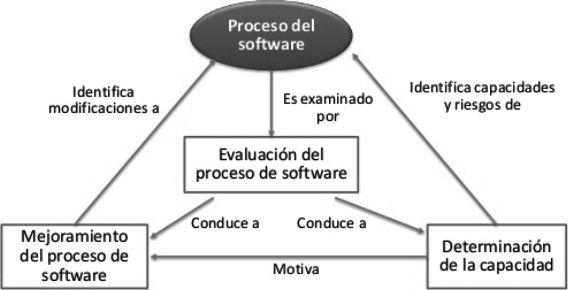
\includegraphics[width=0.7\linewidth]{Resources/evaluacionSoftware}
  \caption{Esquema de la evaluación del proceso software.}
  \label{fig:evaluacionSoftware}
\end{figure}

\subsection{Capability Maturity Model Integration (CMMI)}
Es un modelo que centra su evaluación en las \textbf{áreas del proceso}.\\
Cada área del proceso consta de un conjunto de \textbf{metas específicas} a alcanzar en esa área, además de un conjunto de \textbf{metas globales} que aplican a todas las áreas.\\
Existen dos versiones del modelo:

\paragraph{Modelo continuo} Define el nivel de \uline{capacidad de cada uno de los procesos de la empresa} de manera independiente. Los niveles de capacidad son los siguientes:
\begin{enumerate}
\setcounter{enumi}{-1}
    \item Incompleto.
    \item Realizado.
    \item Gestionado.
    \item Definido.
    \item Cuantitativamente gestionado.
    \item En optimización.
\end{enumerate}

\paragraph{Modelo discreto} Define el nivel de \uline{madurez global de los proyectos} y organizaciones. Proporciona una serie de mejoras concretas que la institución debe pasar para alcanzar el siguiente nivel. 
Para describir el nivel de capacidad usaremos el símil de un conductor en diferentes etapas de su formación:
%El rabo quiere la metáfora del conductor
\begin{itemize}
    \item \textbf{Nivel 1: \textit{Inicial}.} Aprendiendo a conducir.
    \item \textbf{Nivel 2: \textit{Administrado}}. Conductor nobel: sabe conducir y \textbf{reacciona} a los problemas.
    \item \textbf{Nivel 3: \textit{Definido}}. Conductor experto: sabe donde están los problemas y \textbf{proactúa}, tomando las medidas que los reducen.
    \item \textbf{Nivel 4: \textit{Administrado en forma cuantitativa}}. Conductor de autobús: Debe llegar a las paradas a la hora en punto y modificar su velocidad media para lógralo.
    \item\textbf{ Nivel 5: \textit{Optimizando}}. Supera los problemas tratando de averiguar cómo hacer una entrega de Tofu de la manera más rápida posible: \textit{drifting}. % Drifting. sep pues pon drifting. XDDDDD fuera coñas, esto se recuerda mejor así.
\end{itemize}
